\chapter{Ottica geometrica}
\lecture{23}{13 maggio 2024}
L'ottica geometrica si occupa di quali sono i sistemi e le regole con cui si formano le immagini di oggetti a valle di sistemi ottici. Esiste anche un'ottica "non geometrica" che si occupa solo di massimizzare l'intensità di un segnale luminoso a valle di sistemi ottici. Per la lezione di oggi serviranno alcune definizioni:
\begin{description}
	\item[Oggetto (O)]: è un corpo puntiforme o esteso che emette luce o che diffonde la luce di una sorgente. È detto "reale" quando i raggi partono da un punto (es.: oggetto fisico). L'oggetto potrebbe anche essere immagine di un sistema ottico e in tal caso si parla di oggetto virtuale.
	\item[Strumento ottico]: sistema che raccoglie i raggi uscenti da un oggetto e ne modifica la loro direzione.
	\item[Immagine (I)]: figura dell'oggetto realizzata attraverso i raggi deviati dagli strumenti ottici. È detta "reale" se i raggi deviati dallo strumento ottico convergono in un punto, mentre è detta "virtuale" se convergono i prolungamenti dei raggi (es.: specchio).
\end{description}
Gli strumenti ottici che studieremo sono "strumenti ottici stigmatici": i raggi generati da un punto di un oggetto convergono in un punto dell'immagine e i due punti sono detti "punti coniugati". Si ha uno strumento "astigmatico" quando non vi è corrispondenza biunivoca tra punto oggetto e punto immagine.

Si distinguono anche diversi casi di superfici:
\begin{description}
	\item[Superficie catottica] o specchio, quando il fenomeno che si realizza primariamente è quello della riflessione.
	\item[Superficie diottrica] o diottro, quando il fenomeno che si realizza primariamente è quello della rifrazione.
\end{description}
Per gli specchi la legge fisica è particolarmente semplice (\(\theta _i = \theta _r\)) e non dipende dalla pulsazione. Per i diottri è più complicata perché dipende anche dalla pulsazione/lunghezza d'onda. Questo fenomeno è detto "cromatismo" delle superfici diottriche. Si parla di "acromatismo" quando il sistema ottico è studiato in modo da minimizzare questo effetto.

\section{Specchi}
Consideriamo superfici approssimabili come parte di sfera. Per convenzione il raggio \(R\) è positivo se la curvatura è interna allo spazio immagine, mentre è negativo se la curvatura è interna allo spazio oggetto. Faremo riferimento alla seguente figura:
\begin{figure}[H]
	\centering
	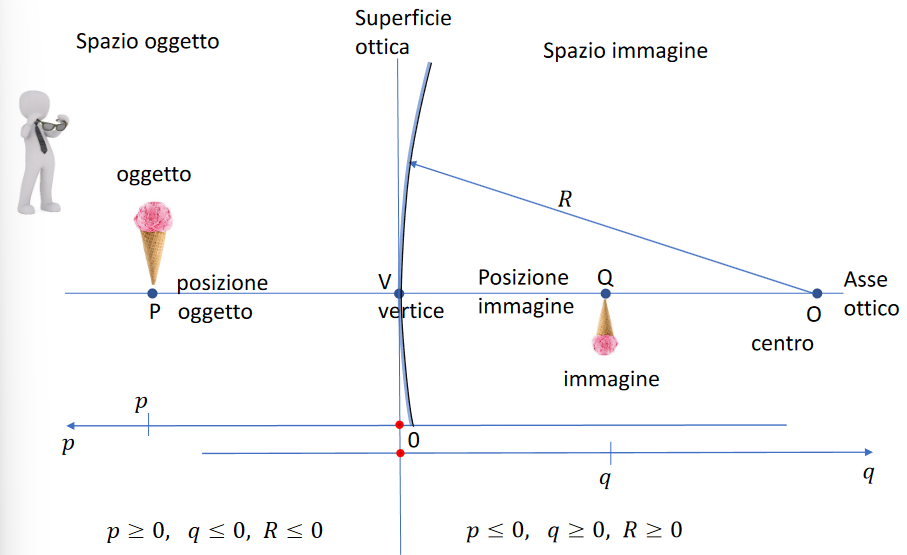
\includegraphics[width=0.6\textwidth]{screenshots/2024-05-13-11-30-35.png}
\end{figure}
Facendo tendere \(O \to \infty \), lo specchio diventa uno specchio piano. I raggi che partono da P nello spazio oggetto e si riflettono sullo specchio piano, se prolungati, convergono nel punto Q appartenente allo spazio immagine. Quindi lo specchio è una superficie stigmatica. Introducendo un altro punto P' si nota che le distanze vengono mantenute dallo specchio piano:
\begin{figure}[H]
	\centering
	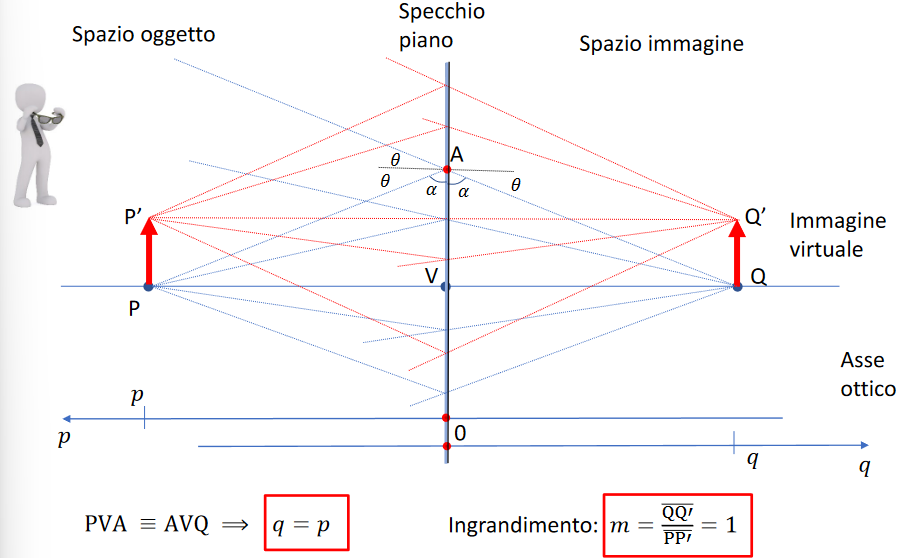
\includegraphics[width=0.6\textwidth]{screenshots/2024-05-13-11-38-55.png}
\end{figure}
Consideriamo ora una porzione di superficie sferica a specchio. Se è convessa, \(R>0\), se è concava \(R<0\). Per costruire le immagini si tracciano alcuni raggi particolari: paralleli all'asse ottico, passanti per il vertice, passanti per centri di curvatura, fuochi, ecc... Nelle superfici stigmatiche questi raggi che partono dal punto P convergono (se prolungati) in un punto Q coniugato a P.

\subsection{Specchio concavo}
Studiamo la seguente figura:
\begin{figure}[H]
	\centering
	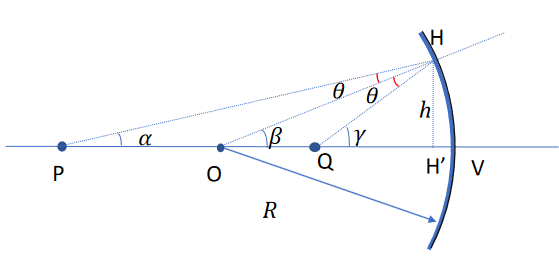
\includegraphics[width=0.5\textwidth]{screenshots/2024-05-13-11-44-29.png}
\end{figure}
Osservando la figura si ottiene che \(\alpha + \theta = \beta \), \(\beta + \theta = \gamma \), da cui \(\alpha + \gamma = 2 \beta \). Approssimiamo per angoli piccoli: siano \(\tan \alpha = \quotient{HH^{\prime} }{PH^{\prime} } \implies \alpha \thickapprox \frac{h}{p} \), \(\tan \beta = \quotient{HH^{\prime} }{OH^{\prime} } \implies \beta \thickapprox \frac{h}{\vert R \vert }= -\frac{h}{R} \), \(\tan \gamma = \quotient{HH^{\prime} }{QH^{\prime} }\implies \gamma \thickapprox \frac{h}{\vert q \vert }=-\frac{h}{q} \) dove i cambi di segno sono dovuti al fatto che siamo nello spazio oggetto e che lo specchio è concavo. Otteniamo quindi
\begin{gather}
	\alpha + \gamma = 2\beta \implies \frac{h}{p} - \frac{h}{q} = -\frac{2h}{R}\\
	\frac{1}{p} - \frac{1}{q}= - \frac{2}{R} \coloneqq -\frac{1}{f}
\end{gather}
\begin{definition}
	[Fuoco dello specchio]
	Nella formula appena scritta si è definito il "fuoco" dello specchio:
	\begin{equation}
		f=\frac{R}{2}
	\end{equation}
	Si avrà \(f<0\) per uno specchio concavo e \(f>0 \) per uno specchio convesso.
\end{definition}
Il fuoco ha la proprietà di essere il punto in cui convergono i raggi generati da punti con \(p\to +\infty \). Questi punti dividono lo spazio in quattro parti: per P a sinistra di O, Q sarà tra O ed F; per P tra O e F, Q sarà a sinistra di O; per P tra F e V, Q sarà a destra di V; per P a destra di V, Q sarà tra F e V. Studiamo ora l'ingrandimento dovuto a uno specchio concavo di un oggetto a sinistra di O:
\begin{figure}[H]
	\centering
	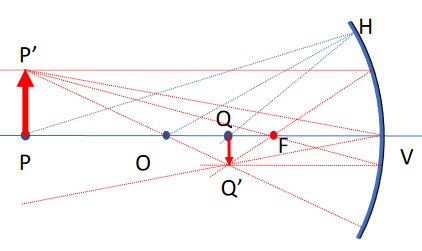
\includegraphics[width=0.4\textwidth]{screenshots/2024-05-13-11-57-01.png}
\end{figure}
VPP' e VQQ' sono triangoli simili, quindi l'ingrandimento è \(m= \frac{QQ^{\prime} }{PP^{\prime} }=\frac{\vert q \vert }{\vert p \vert }= -\frac{q}{p}\). L'immagine è reale, ma è rovesciata. Se ora l'oggetto è tra F e V, la sua immagine sarà virtuale nello spazio immagine. Inoltre sarà ingrandita e diritta. Facendo il disegno si ricava facilmente che
\begin{equation}
	m = \frac{QQ^{\prime} }{PP^{\prime} }=\frac{q}{p}
\end{equation}
Questa costituisce da ora la definizione di ingrandimento. Si avrà \(m> 0\) per un'immagine dritta, \(m<0\) per un'immagine rovesciata.

% TODO: se necessario guarda le slide
\subsection{Specchio convesso}
Per lo specchio convesso si ottengono le stesse formule dello specchio concavo. Si fa il disegno e si ricava facilmente tutto quanto. L'unica differenza è che si avranno \(R<0\) e \(q>0\). Si verifica anche che per P nello spazio oggetto, Q è sempre tra V e il fuoco e che l'ingrandimento è sempre \(0 \leq m \leq 1\).

\section{Diottri}
Si parla di superfici diottriche quando anziché considerare la riflessione si considera la rifrazione. Ovviamente si avrà sempre un po' di riflessione, ma in questo contesto viene trascurata e si studia solo quello che avviene per una superficie diottrica di curvatura sferica.
\begin{figure}[H]
	\centering
	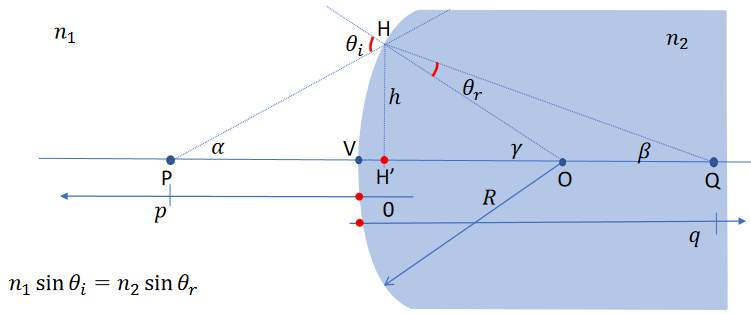
\includegraphics[width=0.5\textwidth]{screenshots/2024-05-13-12-28-42.png}
\end{figure}
L'immagine in Q è reale perché ottenuta dai raggi stessi e non dal loro prolungamento. Per angoli piccoli si approssima \(n_1 \theta _i = n_2 \theta _r\). Si ha inoltre \(\alpha + \gamma = \theta _i\) e \(\beta + \theta _r = \gamma \), da cui \(n_1 (\alpha + \gamma )=n_2(\gamma -\beta )\). Operiamo le stesse approssimazioni di prima:
\begin{figure}[H]
	\centering
	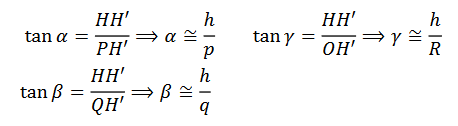
\includegraphics[width=0.4\textwidth]{screenshots/2024-05-13-12-33-50.png}
\end{figure}
Così si ricava che
\begin{gather}
	n_1 \left( \frac{h}{p} +\frac{h}{R} \right) = n_2 \left( \frac{h}{R} - \frac{h}{q} \right)\\
	\frac{n_1}{p} + \frac{n_2}{q} = \left( \frac{n_2 - n_1}{R} \right)   
\end{gather}
Se \(p\to +\infty \), \(q=\frac{n_2}{n_2 -n_1}R \coloneqq f_2\). Se \(q \to +\infty\), \(p=\frac{n_1}{n_2 - n_1}R \coloneqq f_1\). Con queste definizioni la formula trovata diventa
\begin{equation}
	\frac{f_1}{p}+\frac{f_2}{q}=1
\end{equation}
Costruisco l'immagine attraverso il diottro sferico:
\begin{figure}[H]
	\centering
	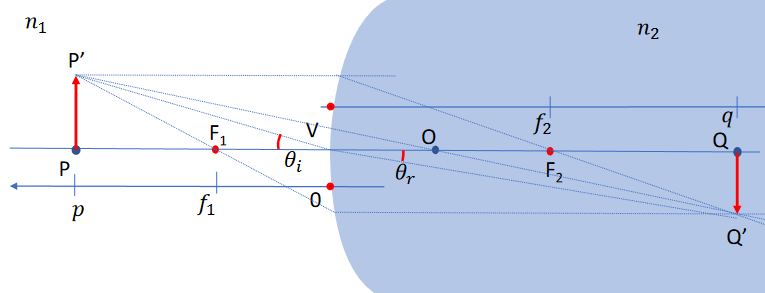
\includegraphics[width=0.6\textwidth]{screenshots/2024-05-13-12-42-26.png}
\end{figure}
I triangoli OPP' e OQQ' sono simili, quindi l'ingrandimento è \(m=\frac{QQ^{\prime} }{PP^{\prime} }=\frac{QO}{PO}=\frac{q-R}{q+R}=\frac{n_1 QV}{n_2 PV}= \frac{n_1 q}{n_2 p}\).

\subsection{Lenti spesse}
Consideriamo un sistema ottico costituito da due superfici diottriche che condividono lo stesso asse ottico. Queste costituiscono una lente, in generale una lente spessa, caratterizzata da due raggi di curvatura \(R_1\) e \(R_2\), un indice di rifrazione e uno spessore \(L\).
\begin{figure}[H]
	\centering
	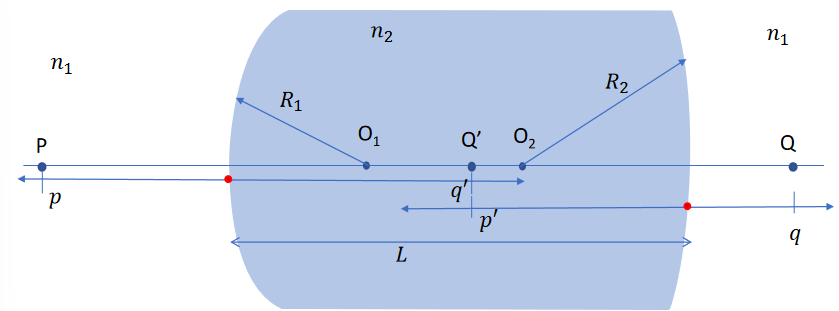
\includegraphics[width=0.6\textwidth]{screenshots/2024-05-13-12-49-19.png}
\end{figure}
Usando quanto ricavato per i diottri si trova che
\begin{align}
	\frac{n_1}{p} + \frac{n_2}{q^{\prime} } &= \left( \frac{n_2 - n_1}{R_1} \right) &
	\frac{n_2}{p^{\prime} } + \frac{n_1}{q} &= \left( \frac{n_1 - n_2}{R_2} \right) 
\end{align}
con \(q^{\prime} + p^{\prime} = L\). Approssimiamo per angoli piccoli e consideriamo lenti sottili (\(L\to 0 \implies p^{\prime} =-q^{\prime} \)).
\begin{figure}[H]
	\centering
	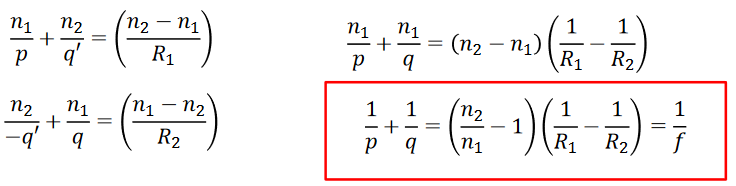
\includegraphics[width=0.5\textwidth]{screenshots/2024-05-13-12-54-30.png}
\end{figure}
\(f\) è detta "distanza focale" della lente, \(D=\quotient{1}{f} \) è detta "diottria" della lente. Per \(p\to +\infty \), \(q=f\). Allo stesso modo, per \(q \to +\infty \) si ha \(p=f\). Se \(f>0\) la lente è detta convergente, mentre se \(f<0\) la lente è detta divergente. L'ingrandimento è identico alla formula vista finora.
\begin{figure}[H]
	\centering
	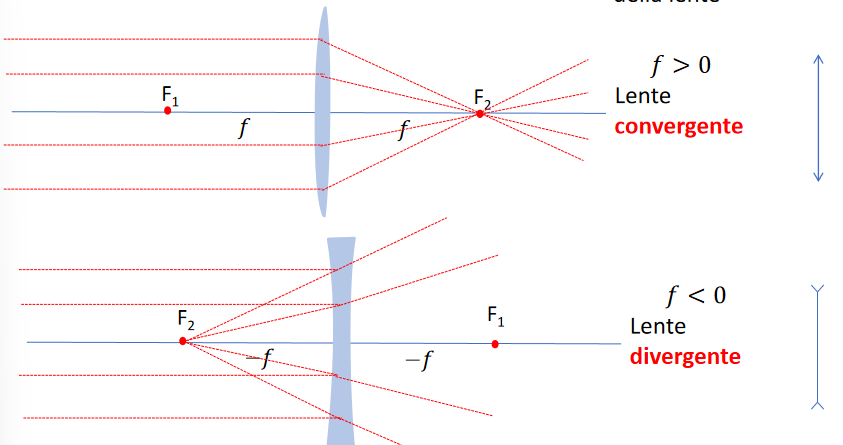
\includegraphics[width=0.5\textwidth]{screenshots/2024-05-13-13-00-49.png}
\end{figure}
Per la costruzione di immagini dobbiamo ricordare tre tipi di raggi importanti: paralleli all'asse ottico nello spazio oggetto (convergono in F2), passanti per V (proseguono dritti) e passanti per F1 (escono paralleli all'asse ottico nello spazio immagine).